\documentclass[journal, letterpaper]{IEEEtran}
\usepackage{listings}
\usepackage{fancyvrb}
\usepackage{framed}
\usepackage[listings,skins]{tcolorbox}
\usepackage[skipbelow=\topskip,skipabove=\topskip]{mdframed}
\usepackage{pbox}
\usepackage{graphicx}
\usepackage{url}
\usepackage{hyperref}
\usepackage{caption}

\mdfsetup{roundcorner=0}
% Congyang: Added the geometry module to add the margin of bottom
\usepackage[top=1in, bottom=1.2in, left=0.7in, right=0.7in]{geometry}
% Congyang: Added the indent first module (and delete "\\" of every paragraph) to make it indent every paragraph.
\usepackage{indentfirst}

\begin{document}
\title{Optimizing Hubway Bicycle Docks Allocation in Boston City}
% Congyang: Title Or: Boston Hubway Bicycle Sharing System Facility Allocation Analysis (choose a fit)
\author{Congyang Wang, Fangyu Lin, Meng Li \\ Department of Computer Science, Department of Data Science -- Worcester Polytechnic Institute, MA, 01609 \\ Email: \{cwang8, flin, mli6\}@wpi.edu}
% Congyang: Added our emails
\maketitle

% The Abstract
\begin{abstract} 
\large As the number of people living in Boston grows, the traffic environment has become more and more crowded. In recent years, local government has already built up the bicycle system to ameliorate traffic conditions and create a green environment. The idea is to design and implement a bicycle system that is accessible and convenient to the public by planning station locations satisfying the public needs. Residents can rent a bike from one Hubway station and return it at another Hubway station which is closed to their destinations. However, it is important and challenging for the government to arrange the number of bicycle docks between stations appropriately so that the system can benefit almost everyone and balance traffic flows in Boston as much as possible. Our approach is to arrange bicycle docks for each station such that maximizes the coverage of the bicycle system and increase penetration of bicycle usage, based on the Hubway shared bike data in Boston Area between 2011 and 2013. Fortunately, the total number of capacity for each Hubway station in Boston area is known, we are going to estimate available bikes from historical Hubway bike trips data, which contains information on stations and every trip. Our goal is to optimize the number of docks for each Hubway station to satisfy the demands and supplies, and at the same time to mitigate traffic congestion as well as to create a green environment in Boston Area. 
\end{abstract}

% The Keywords 
\begin{IEEEkeywords}
Bike-sharing program;
Bike-station location;
Location Optimize model;
\end{IEEEkeywords}

\section{Introduction}
\large
Sustainable living and energy conservation have been populous across the globe in recent decades since now people are aware of severe damage on environment inflicted by industrialization. To promote renewable energy, a significant number of developed countries launched a shared bicycle program in the hope that it will facilitate people to switch to green transportation. The Hubway is such program launched by Boston government in 2011 with 61 stations and 600 bicycles initially. By the end of 2013, the system has been expanded to 130 stations and 1200 bicycles. However, the current Hubway system is designed mainly for entertainment purpose. Obviously, the bicycle system has far more benefits than just for fun. It even has high potentials to solve urban problems of oversized and overpopulated cities, for instance, traffic congestion, air pollution, etc. 

To explore more potentials usage of Hubway Shared Bike, a new bicycle facility plan has to be designed based on trip demands, regardless of trip purposes. As a consequence, the new system will be more efficient and attractive compared to the current one as well as produce more beneficial outcomes. In the first place, reasonable bicycle facility planning will increase the usability of the system and correspondingly reduce usage of private automobiles and emission of carbon dioxide. Plus, the decline in consumption of fossil fuels will help to conserve the non-renewable resources. Secondly, traffic congestion will be mitigated if people switch to bicycles from automobiles. For low-income residents, the Hubway system can provide them an alternative and healthy commute travel solution. For college students, cycling is also a cost-effective and flexible option which better fits their school schedules compared to the subway. Additionally, an efficient bicycle system is likely to ease mass transit pressures for a metropolis.  

However, optimizing the entire design, including location planning of stations and re-allocation of docks and bicycles, requires multiple data sources, such as trip records and GIS information, and is way too large for a one-month project. To tailor it to meet workload that we can handle in half semester, the problem is simplified to optimize station capacities based on trip demands and current design. In other words, our goal is to modify current design with the least efforts and costs, focusing on re-allocation of docks for stations so that the hubway system can satisfy public demands as much as possible. To minimize costs of optimizing the re-allocation of docks, the total number of docks is kept untouched. To tackle the problem, we will use a dataset of the Boston Hubway 2011 Trips And Stations.  Figure[1] shows the Hubways Station in the Boston Area. 

%To tackle the problem, we are going to use a dataset of the Boston Hubway 2011 Trips And Stations to predict and optimize the docks for each Hubway station system, which is supposed to be efficient and meet the public trip demands and supplies.

%Basically, we will employ a location-allocation model to select stations such that costs between demand locations and candidate stations are minimized, or coverage of stations is maximized [1]. The dataset will serve a goal of estimating the distribution of potential demands for the location-allocation model.

According to the "Wisconsin Bicycle Planning Guidance Handbook (WBPG)" [2], it is necessary to take both supplies and demands of shared bicycles into consideration in the shared bicycle facility planning. In the paper, we proposed our methodology based on the demands and supplies from the Hubway Bike Trips Data in Boston Area between 2011 and 2013. The rest of paper is organized as follows. Section 2 is the related work in recent years, which talks about what other research projects are doing by using the Hubway Bike Trips Data. Section 3 is going to introduce the Methodology we are proposed, and how can we predict and optimize the docks at each Hubway Stations grouped by Regions. Section 4 Evaluation is going to use the real Hubway Bike Trips data to test our methodology and compare the results with real data. And the last section 5 is the Conclusion for this paper, what we have observed by the Evaluation Experiment results. 

\begin{figure}
  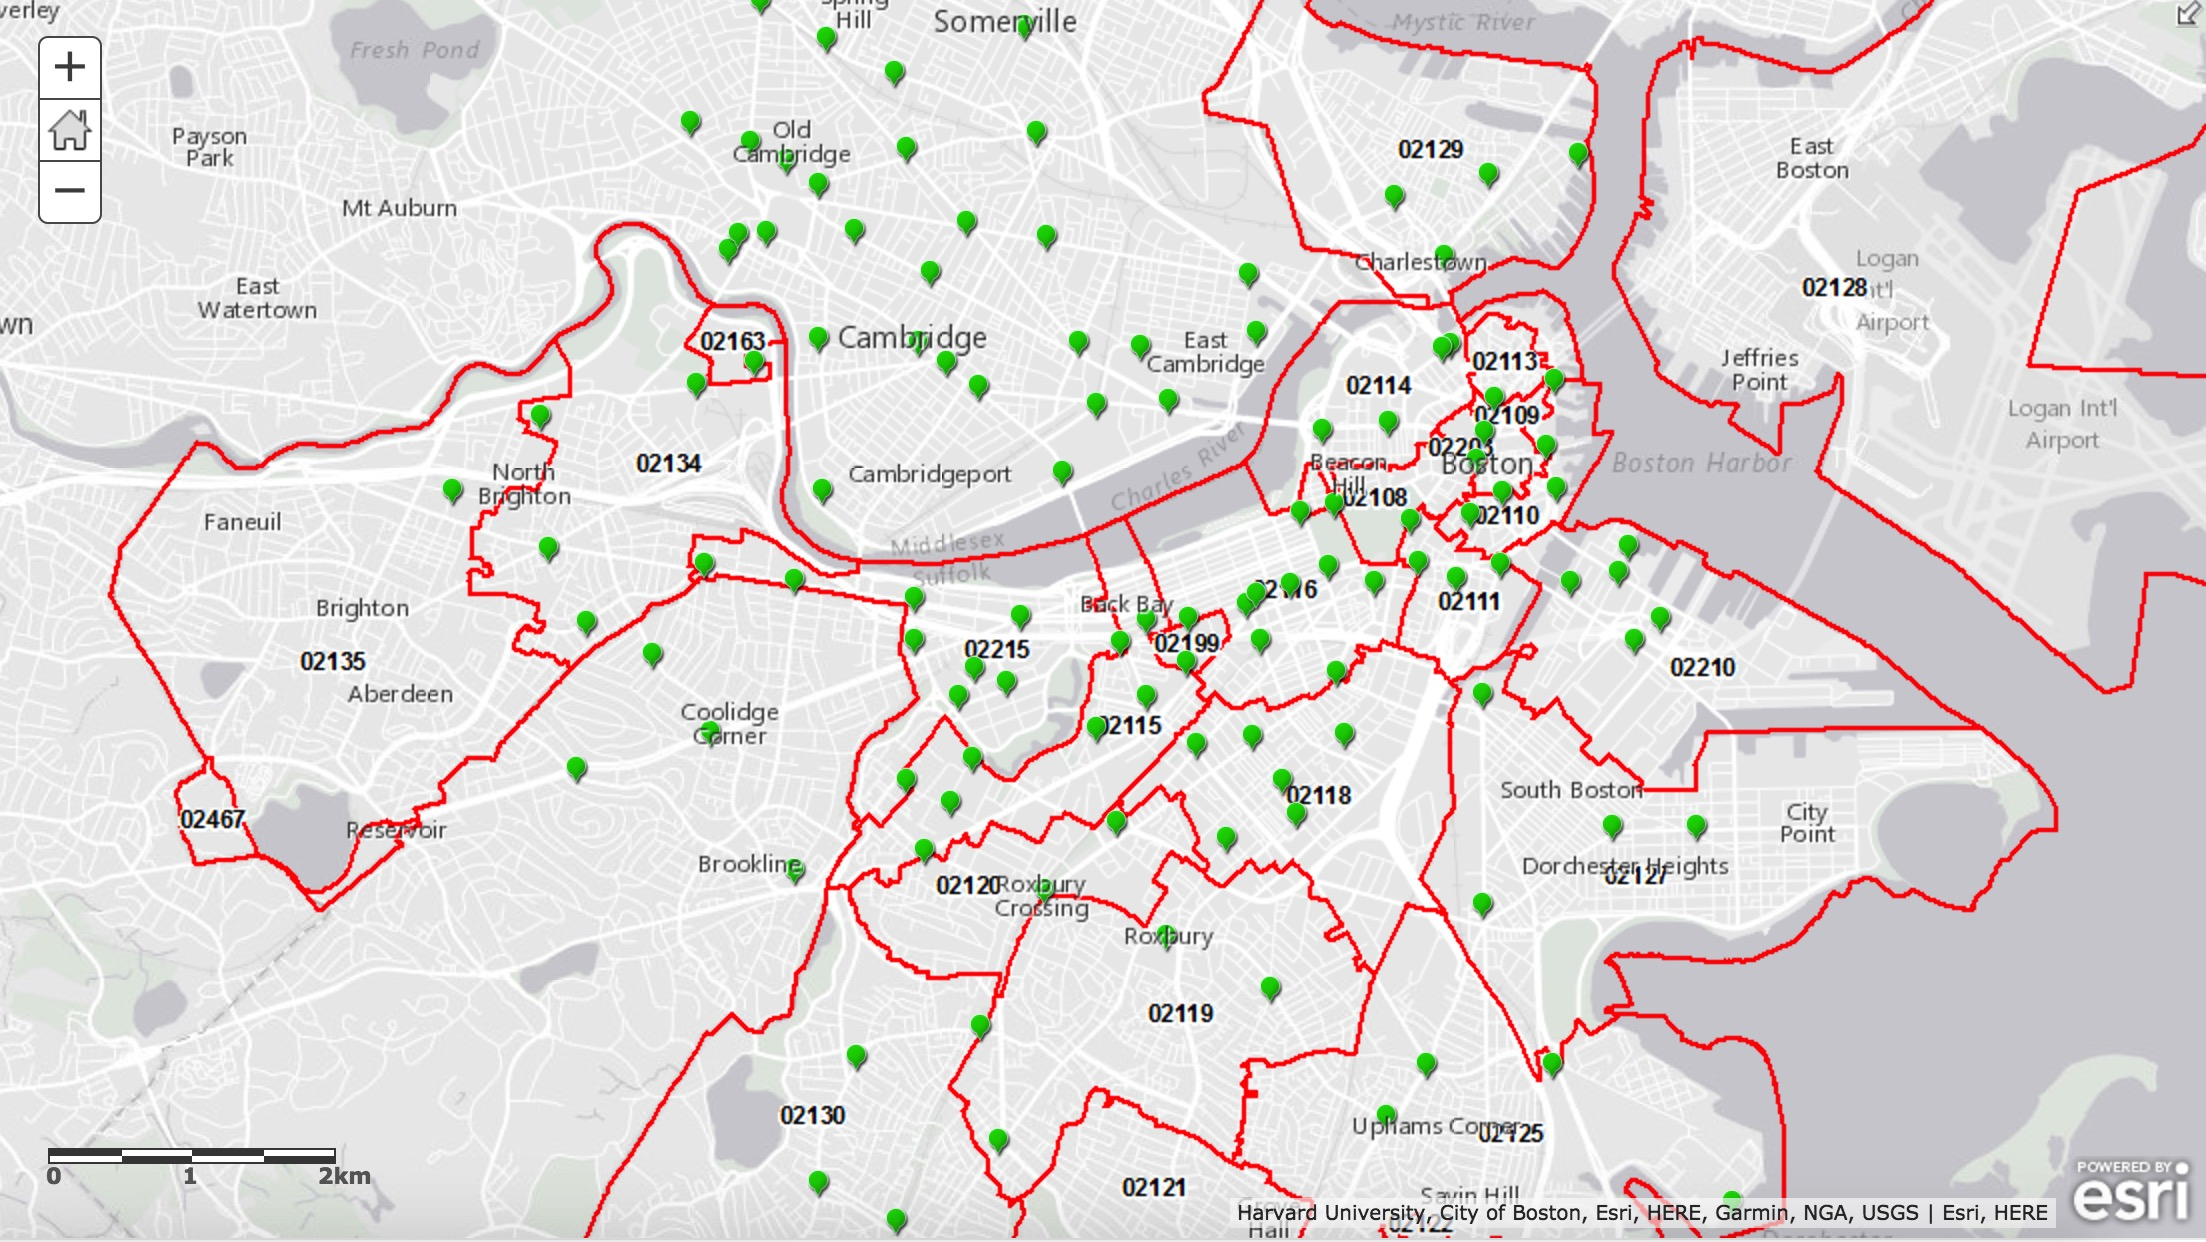
\includegraphics[width=0.5\textwidth]{stationdot.jpg}
  \caption{Hubway Station Location In Boston Area}
  \label{fig:1}
\end{figure}

\section{RELATED WORK}
\large
The research paper we have reviewed currently is the one [3] that analyzes the bike rental system using the P-Median (minimize-impedance solution), which is to minimize "weighted costs between demand points and solution facilities" to maximize coverage. Moreover, in the paper, it uses the "GIS-based multi-criteria analysis tools." As we know, this is a popular tool for data visualization on a map creating a heat map rendering with other features. However, the tool is inadequate and flawed in certain aspects considering our problem. So we are going to apply a more advanced method. To estimate the capacity of each bike station, first, aggregate the number of bicycles rented from one station on a daily basis. Then select the maximum over daily total from each station as the estimated capacity. Regarding accessibility and regional population, some stations will have more bicycles that are rented than others. Based on the estimated needs, we can make a right decision to allocate bikes to stations to maximize overall usage of bicycles. Besides, we are reviewing other methodologies, such as multi-criteria decision analysis and exploratory spatial data analysis. We will make comparisons across them to figure out the best one for our problem and evaluate performance by comparing it with baseline algorithms.

\section{METHODOLOGY}
\large
\subsection{Problem Setting}
Technically, we intend to estimate the number of docks installed at each station that can satisfy demands of the station. To achieve the goal, we propose a two-step framework:
\begin{itemize}

\item Step 1: Predict the number of available bicycles at each station, i.e., the number of bicycles allocated to each station in the very beginning, which meets trip demands of the station. 
\item Step 2: Estimate capacity of each station to accommodate predicted the number of available bicycles, keeping the total number of docks of the entire system unchanged.  
\end{itemize}  

Intuitively, the sum of available bicycles at one station and bicycles that have traveled to it should meet the bicycle demands of the station. On the other hand, each station also has to provide sufficient empty docks to accommodate bicycles that have traveled to the station from other stations. Thus, the number of available bicycles and the capacity of each station should be predicted subject to these constraints. 

The two-step framework is essentially developed to create a dock re-allocation plan taking trip demands into consideration. Since the number of docks at each station is estimated by the number of available bicycles which is predicted by trip demands, the station capacity estimates take trip demands into account spontaneously. In the first step, bicycle demands are predicted with inbound and outbound trips. In the second step, the Great Boston Area is split into 35 regions by zipcodes. Docks are assigned to each region first corresponding to its bicycle demands. For example, suppose the city has two regions $A$ and $B$. Region $A$ accounts for 20\% bicycle demands of the total demands and region $B$ accounts for 80\%. Then 20\% docks of the total will be allocated to the region $A$ and the remaining 80\% docks will be allocated to the region $B$. Within each region, docks are allocated to stations following the same procedure.     

To make notations in our methods simple and clear, following terms are defined. 

$Outbound_{s}$: the number of bicycles outbound from the station $s$.

$Inbound_{s}$: the number of inbound bicycles to the station $s$. 

$Avl_{s}$: the number of available bicycles at the station $s$ in the beginning. 

$Capacity_{s}$: the capacity of station $s$, i.e., the total number of docks at the station $s$. 

To simplify the problems and optimize allocation of bicycles and docks with the lowest costs and the least efforts, we made several assumptions.

\begin{itemize}
\item The total numbers of docks of the bike-sharing system is fixed and equal to the total of the current Hubway system throughout the study.
\item Given trip data with start time and end time, regional population is assumed to be redundant for trip demand forecasts and will not be considered in the study.
\end{itemize} 
\subsection{Bike Demand Prediction For Stations}
Since demands of bicycles are different from station to station, a strategy that distributes bicycles uniformly across all stations as adopted by most of bike-sharing systems is unreasonable. It may create a surplus of bicycles for stations with low demands and a shortage of bicycles for stations with high demands. To balance bicycle supplies and demands across stations, the number of available bicycles in theory should satisfy the equation below,
$$Avl_{s} + Inbound_{s} \ge Outbound_{s}$$

%\subsection{Capacity Prediction For Stations}
%The dock demand is predicted subject to two constraints:
%\begin{itemize}
%\item Every inbound bicycle is assigned an empty dock at a station.
%\item A station has enough docks to park as many bicycles as demanded when the demands reach the highest level.
%\end{itemize}

%$$Capacity_{s} - Avl_{s} = Inbound_{s} - Outbound_{s}$$

%The left hand side of the equation is the number of empty docks and the right hand side is the number of bicycles that have to be parked at the station. The rationale behind the equation is that each station must have adequate empty docks so that every bicycle at the station can be parked with a dock. Meanwhile, when a station reaches its full capacity, in other words, no docks are empty, it should satisfy the highest bike demands, i.e., 
%$$Capacity_{s} \ge max(Outbound_{s})$$

%In a special case when a station has no outbound bicycles, it should be able to accommodate all inbound bicycles and bicycles that are allocated to the station initially, i.e., 
%$$Capacity_{s} \ge max(Inbound_{s}) + Avl_{s}$$
\begin{figure*}
  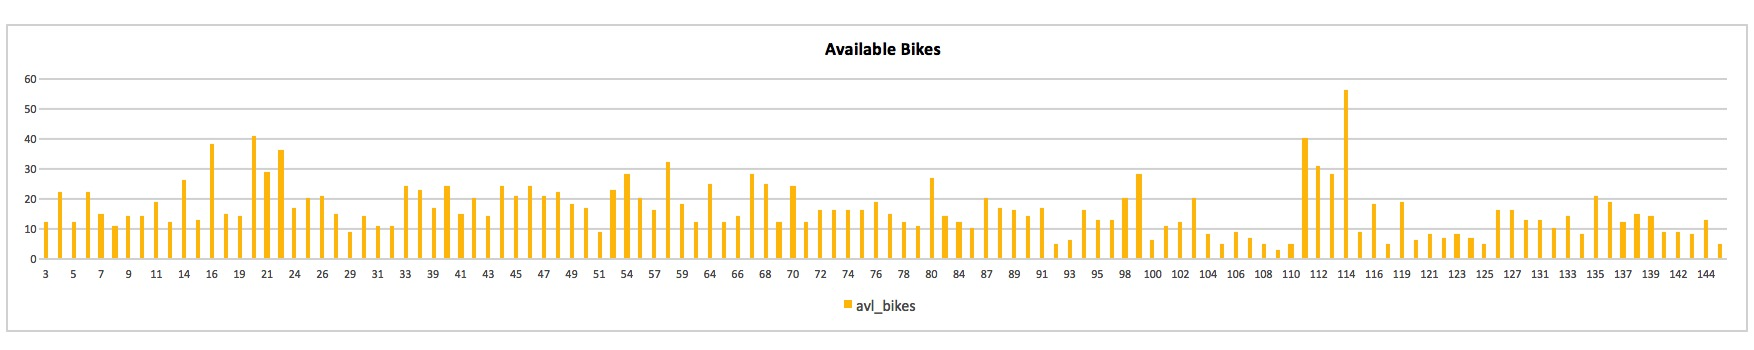
\includegraphics[width=1\textwidth]{availablebike.jpg}
  \caption{Docks Re-allocation Result Plot}
  \label{fig:2}
\end{figure*}

\subsection{Estimation Of Dock Allocation}
Since capacity and quantity of available bicycles at each station of the current Hubway System are known, and the totals of docks and bikes are assumed unchanging, the total of docks and bicycles across the city can be obtained. 

With predicted bike demands of individual stations, a demand ratio of bikes at a given region $r$ can be calculated as, 
$$Ratio_{r}^{Bike} = \frac{Predicted \ Avl_{r}}{\sum_{i=1}^{n}Predicted \ Avl_{i}}$$
%$$Ratio_{r}^{Dock} = \frac{Predicted \ Capacity_{r}}{\sum_{i=1}^{n}Predicted \ Capacity_{i}}$$
where $n$ is the number of regions in the Great Boston Area.

For region $r$, dock allocation should follow
%$$Estimated \ Avl_{r} = Ratio_{s}^{Bike} * \sum_{i=1}^{n}Avl_{i}$$
$$Estimated \ Capacity_{r} = Ratio_{r}^{Bike} * \sum_{i=1}^{n}Capacity_{i}$$
where $Capacity_{i}$ are data of the current system.

For a specific region $r$, dock allocation for a station $s$ located in the region is estimated as,
$$Ratio_{s}^{Bike} = \frac{Predicted \ Avl_{s}}{\sum_{i=1}^{m}Predicted \ Avl_{i}}$$
where $m$ is the number of stations in the region $r$.
$$Estimated \ Capacity_{s} = Ratio_{s}^{Bike} * Capacity_{r}$$
where $Capacity_{r}$ is the number of docks in region r estimated previously. 

%\subsection{Time Window}
%Prediction results may change when different time horizon is chosen, since daily $max(Inbound_{s})$, weekly $max(Inbound_{s})$ and monthly $max(Inbound_{s})$ probably are not identical. In our analysis, data will be aggregated on a daily basis, a weekly basis, a monthly basis and a yearly basis. Also, comparisons of accuracy of results produced with four horizons will be performed.
\subsection{Data}
The analysis is conducted with three datasets: hubway\_stations.csv, hubway\_trips.csv, and the most important and the largest data file, stationstatus.csv. Key attributes are summarized below, 
\begin{table}[ht]
%\caption{} % title of Table
\centering % used for centering table
\begin{tabular}{c| c| c} % centered columns (4 columns)
\hline\hline %inserts double horizontal lines
Attribute & Data Type & Description Of Usage  \\  % inserts table
%heading
\hline % inserts single horizontal line
seq\_id (sid) & Character (Primary key) & trip index, counting trips  \\ % inserting body of the table 
\hline
hubway\_id & Character (Reference key) & \pbox{20cm}{Classification for \\ station count sum}  \\
\hline
start\_station & Integer & Demand-based counter  \\
\hline
end\_station & Integer & Supply-based counter   \\
\hline
start\_date & Timestamp & \pbox{20cm}{Classification for \\ day, week, month, year}  \\  % [1ex] adds vertical space
\hline
end\_date & Timestamp & \pbox{20cm}{Classification for \\ day, week, month, year} \\
\hline
zip\_code & Character & Classification for regions \\
\hline %inserts single line
\end{tabular}
\label{table:nonlin} % is used to refer this table in the text
\end{table}

\section{EXPERIMENTS}
\large
%aa\\
\subsection{Data Preparation}
First of all, for the data we are using, which is the Hubway bikes shared trip data in Boston. We assume that the user information is not useful in this paper. It is necessary to simplify the data file before doing the data analysis. First, we are going to delete column with attribute 'subs\_ctype', 'zip\_code', 'birth\_data', and 'gender'. Second, load the data into a database for further calculation. 

Second, the other datafile that we are going to use has the Hubway Station information, which contains the removed bike stations. In this case, we assume that removed Hubway station is no longer available, so we use a filter to remove those stations data. 

Third, the last datafile that we used has information of docks number. We extract a couple of useful columns from this file to do the optimization, which is to group by regions (zipcode) and re-allocate docks for each station in the same region. 

\subsection{Prediction of Available Bikes}
First, group by the station number as well as the start\_date for one table. 
Second, group by the station number as well as the start end\_date for another table.
Third, join the two tables with same station number and subtract the end\_date to the start\_date. 
The result table has three attributes, which are station\_ID, Date, and the number of bikes needs at the station on each date. Next, we find the max number of needs for each station, which means that gets the biggest number through all dates in one station. The result table plot into graph which is shown in Figure[2].

\subsection{Hubway Docks Re-allocation}
In this section, we are using the predicted needed bikes in the previous section to re-allocate the bike dots for each station. We need another data file "stationstatus.csv" which contains the docks numbers for 145 stations. Second, we join the previous table results by the same primary key and foreign key, which are station\_ID number. 
First, we are going to do a ratio of each station in a same group of the region, which is group by zip-code. The result table is shown in the figure[3]. 
Second, use the methodology to re-allocate each station, but the sum of total stations in each region is constant. 
Third, compare the new docks number in each station. The final re-allocation results are ploted in the figure[5]. 
From this graph, we can find out some stations have good dock numbers, but some have to re-allocate to satisfied the requirement of a minimum of demands. 

\subsection{Result Analysis}
According to the results in each plot, our design matches the real situation in Boston Area. For example, the minimum Docks Required to be added at "TD Garden - Causeway at Portal Park \#1" is at least 33 docks. As it is known that TD Garden is a multi-purpose arena which can be used as a BasketBall Field as well as a ice rink and for other entertainment. Also, it is a commuter rail point, connecting inter-city trains and the subway. As a consequence, trip demands at TD Garden are ought to be high, which is consistent with our optimization results: the minimum 33 docks have to be installed. On the other hand, there are some area has redundant docks which is wasting the resources. For example, the Hubway Station at "Jackson Square T at Centre St" has about 14 empty docks. As we known from the map that this Hubway Bike Station is associated with Subway Station. However, from the result we know that people may not want use the Hubways bikes here becasue it is too close for a walking distance to the activities area. In this case, we plan to re-allocate those 14 docks to other Hubways stations. Those are two extreme results which show the correct re-allocation results from our experiment. The figure[4] shows the Heat Map of Docks Re-allocation Result in Boston Area. As we can see directly from the Map that most docks are re-allocated to Boston Downtown Area. Our goal to optimize Hubway Docks for each Station has been achieved.

\begin{figure}
  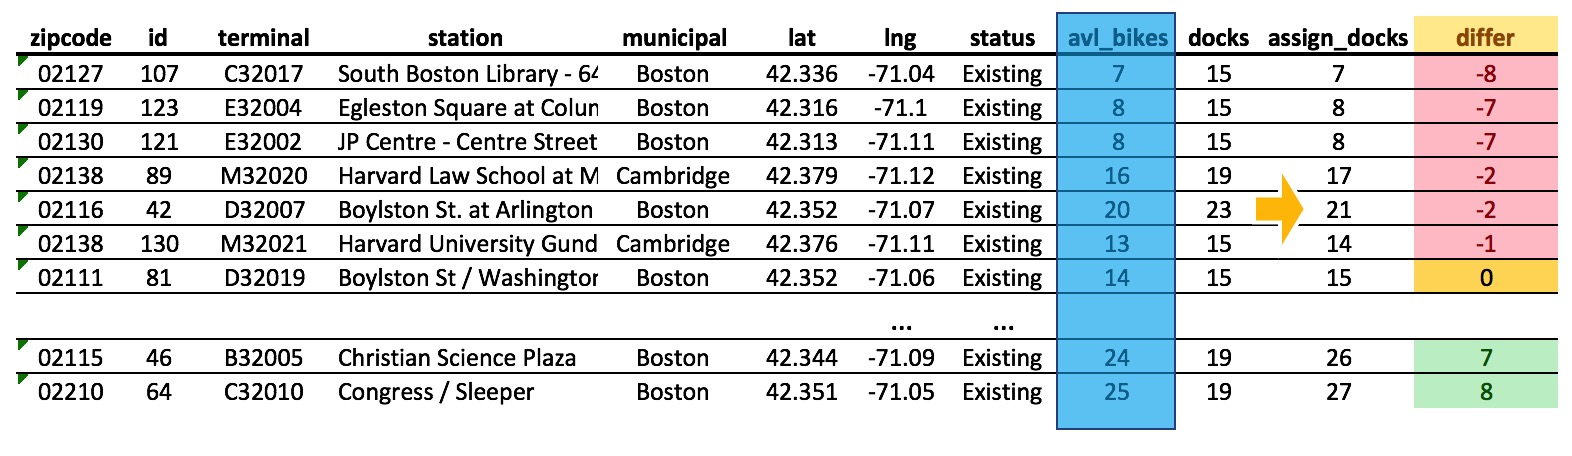
\includegraphics[width=0.5\textwidth]{resultsheet.jpg}
  \caption{Hubways Docks Re-allocation Results}
  \label{fig:3}
\end{figure}   

\begin{figure}
  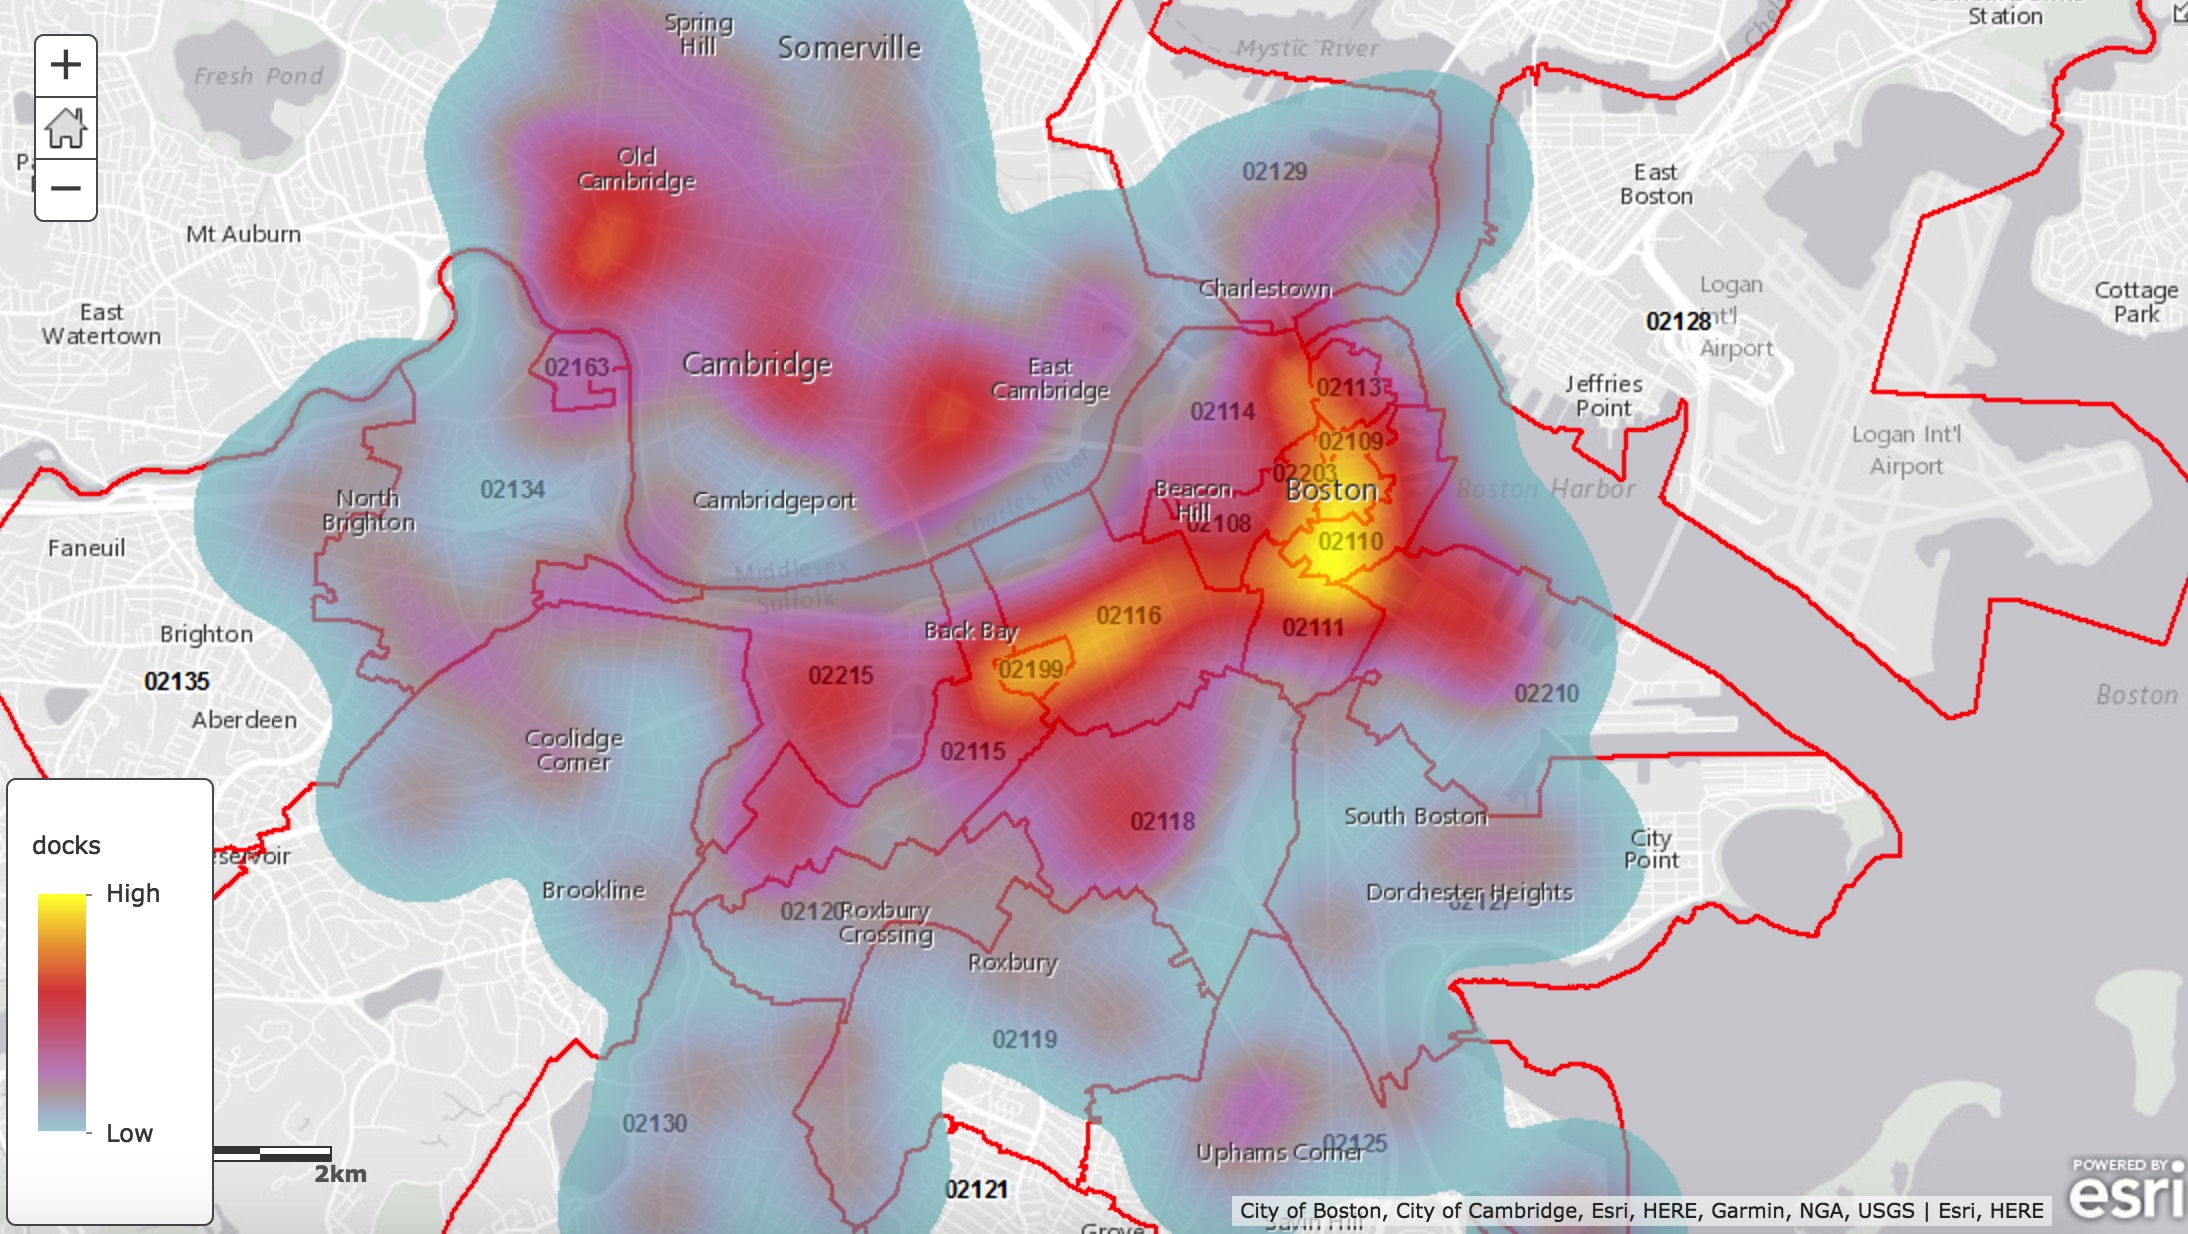
\includegraphics[width=0.5\textwidth]{docksheat.jpg}
  
  \vspace{0.5cm}
  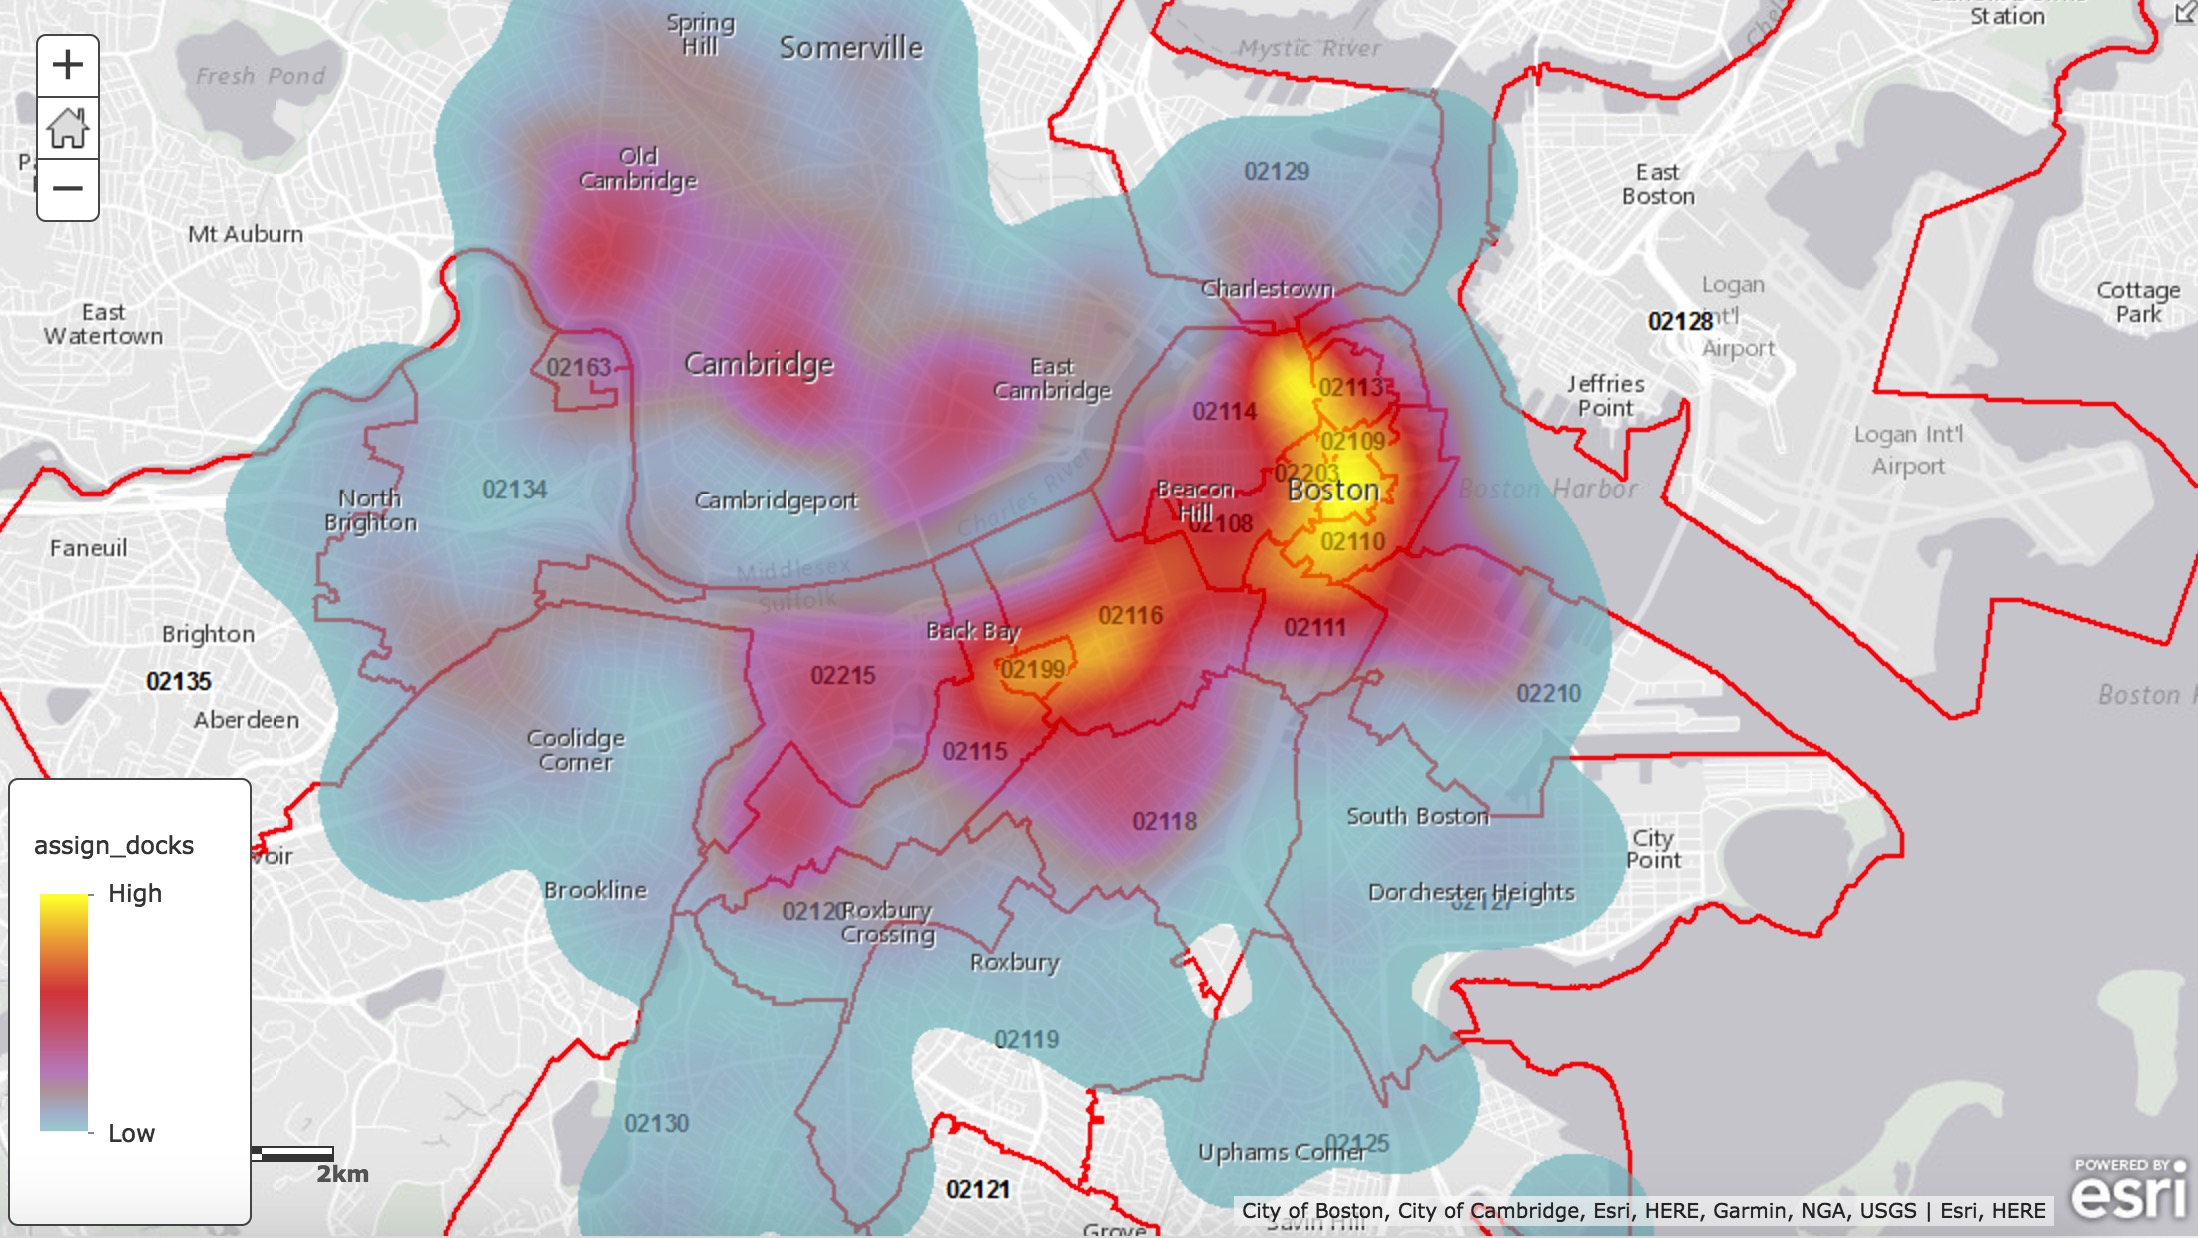
\includegraphics[width=0.5\textwidth]{assigndocksheat.jpg}
  \caption{Heat Map of Docks Re-allocation Result}
  \captionsetup{justification=centering}
  \label{fig:4}
\end{figure}

%%\section{RELATED WORK}
%%\large
%aa\\


\begin{figure*}
  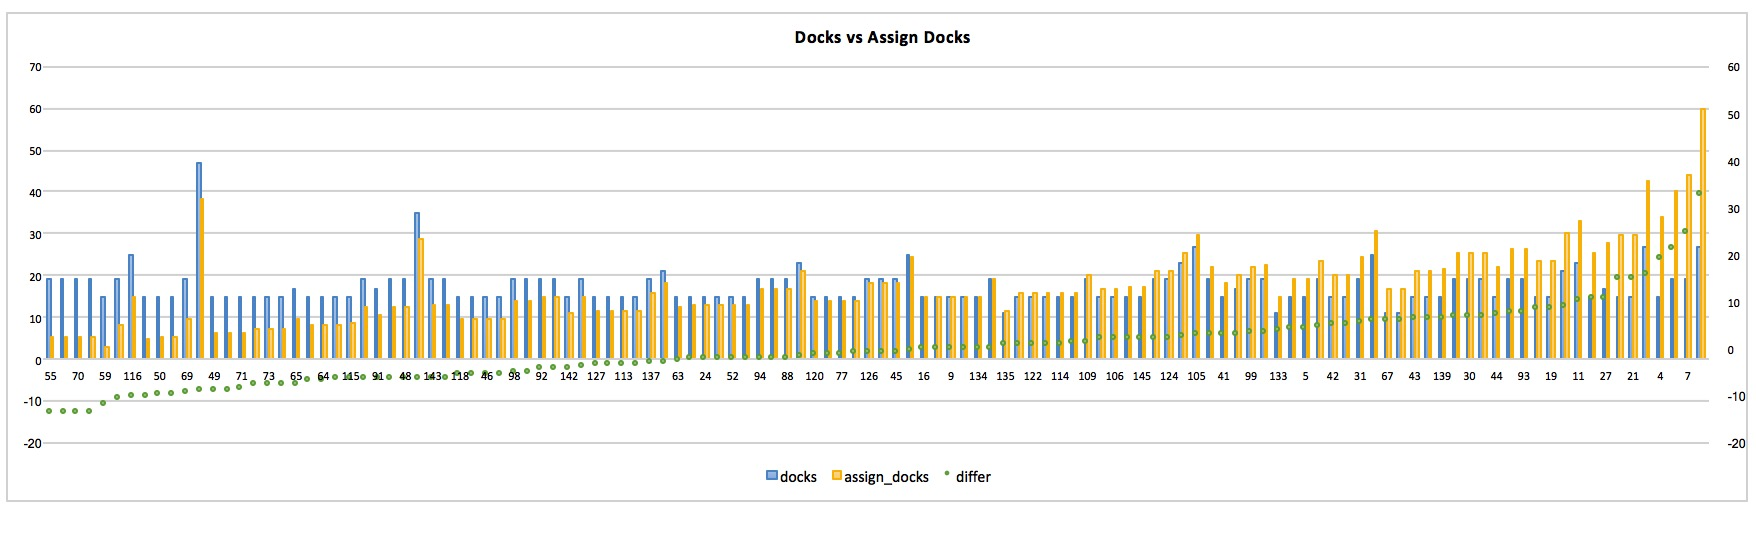
\includegraphics[width=1\textwidth]{dockvsassigndock.jpg}
  \caption{Docks Re-allocation Result Plot}
  \label{fig:5}
\end{figure*}

\section{CONCLUSIONS}
\large
%\\
The goal of this paper is to predict the shared bikes need and re-allocate the Hubway Docks in each station to satisfied the minimum requirement of the demands for that stations by day. The data we used in the paper is from the Hubway Shared Bikes in Boston from 2011 to 2013.  We develop our Methodology to predict the numbers of bikes in each station needs to satisfied the minimum demand for a day. The evaluation results are shown as expected that many Hubway Docks required re-allocation due to a different ratio between "Needs" and "Docks." For the future work, it may be a good practice to make the Docks motivative. It means that each dock can be installed and uninstalled easily in real practice. Use the real Hubway Shared Bike data in Boston, and we can re-allocate the docks dynamically each Months. And this is also an open challenge to use the real-time bike sharing date to re-allocate the docks for each station dynamically in the future. 


\begin{thebibliography}{99}

\bibitem{c1} J. C. García-Palomares, J. Gutiérrez, and M. Latorre, "Optimizing the location of stations in bike-sharing programs: A GIS approach," Applied Geography, vol. 35, no. 1, pp. 235-246, 2012.
\bibitem{c2} Tom Huber, "WISCONSIN BICYCLE PLANNING GUIDANCE" Unpublished, 2003.
\bibitem{c3} N. Baird and D. Kim, "Bicycle Facility Demand Analysis using GIS," Spaces and Flows: An International Journal of Urban and ExtraUrban Studies, vol. 1, no. 2, pp. 1-14, 2011.
\bibitem{c4} G. Rybarczyk and C. Wu, "Bicycle facility planning using GIS and multi-criteria decision analysis," Applied Geography, vol. 30, no. 2, pp. 282-293, Apr. 2010.
\bibitem{c5} I. Frade and A. Ribeiro, "Bicycle Sharing Systems Demand," Procedia - Social and Behavioral Sciences, vol. 111, pp. 518-527, Feb. 2014.
\bibitem{c6} {WinNT, {{ Bamboo Bicycles Beijing} David Wang}, howpublished = {\url{https://www.bamboobicyclesboston.org/}},{Accessed: 2017-02-20}}

\end{thebibliography}

\end{document}